\section{Поверхность потенциальной энергии межмолекулярного взаимодействия}

\begin{figure}[!h]
	\hspace*{-1.2cm}
	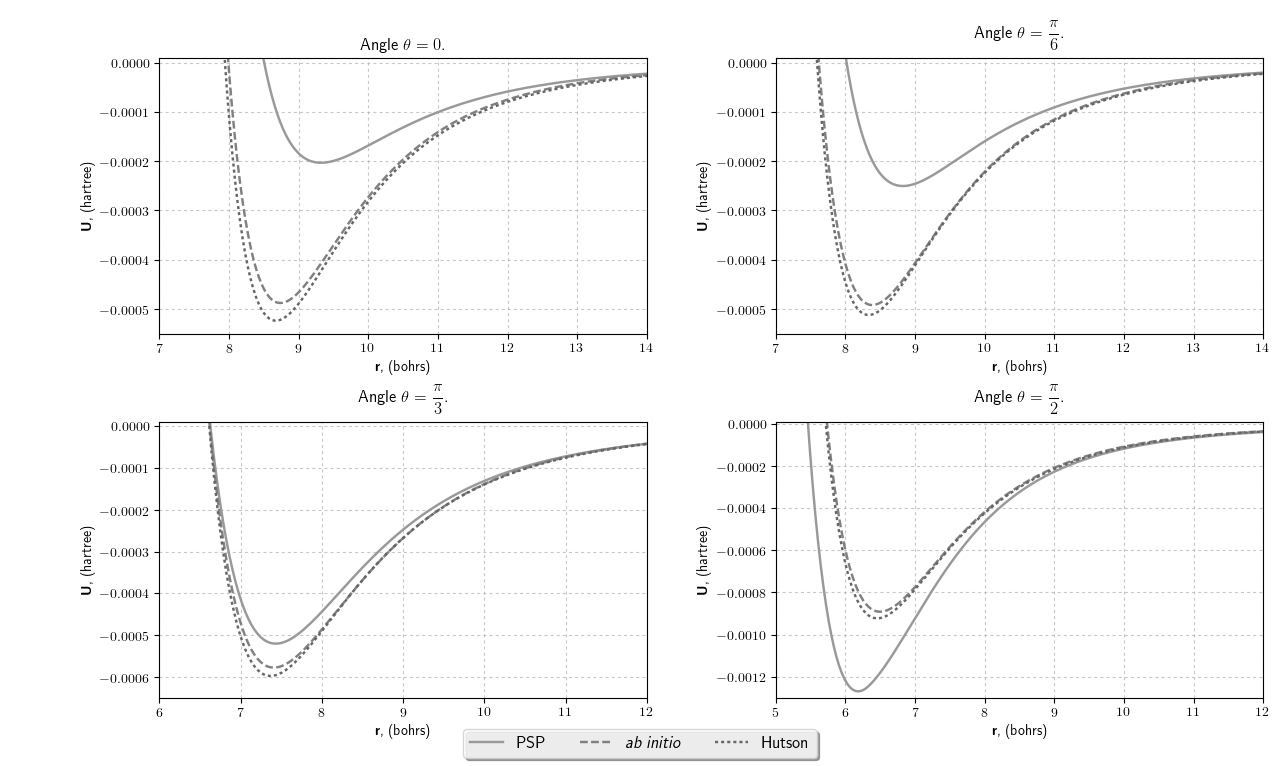
\includegraphics[width=1.1\textwidth]{pictures/potential_well.png}
	\caption{Сечения поверхностей потенциальной энергии при разных углах $\theta$ в области потенциальной ямы.}
\end{figure}

\begin{figure}[!h]
	\hspace*{-1.2cm}
	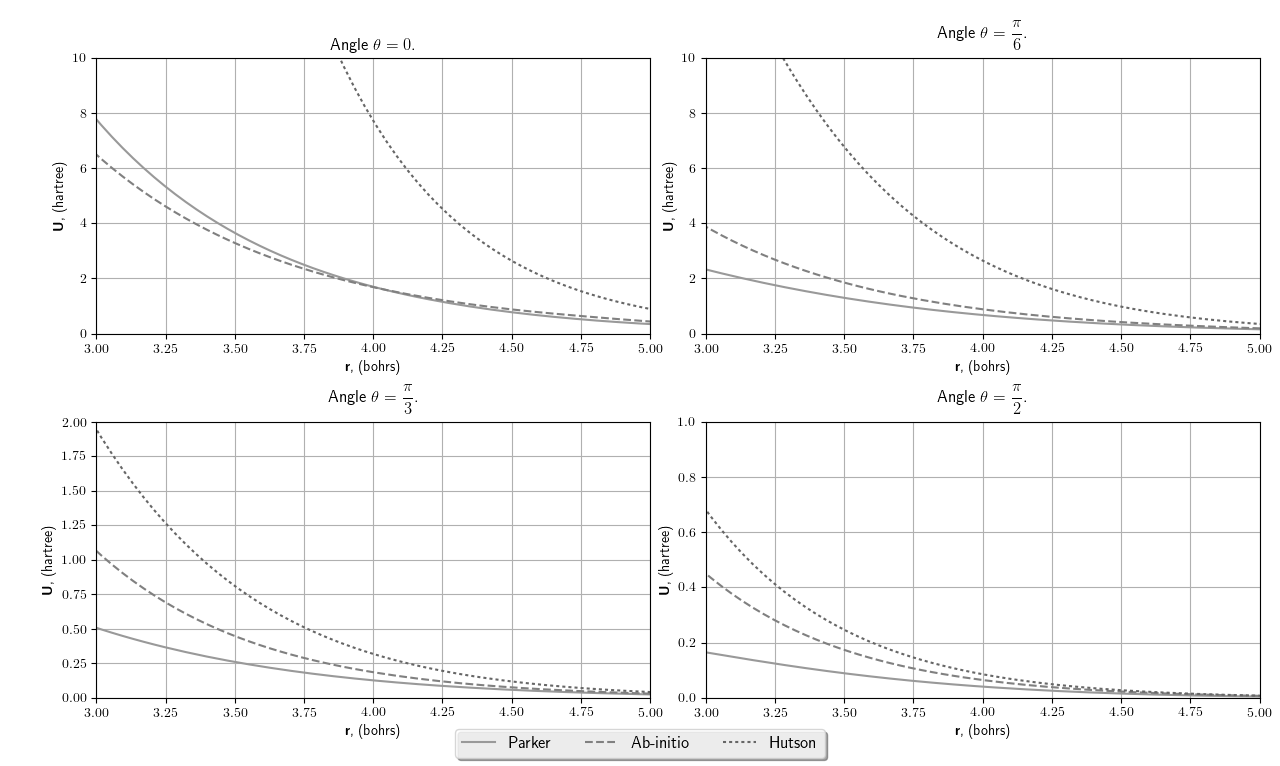
\includegraphics[width=1.1\textwidth]{pictures/potential_wall.png}
	\caption{Сечения поверхностей потенциальной энергии при разных углах $\theta$ в области потенциальной стены.}
\end{figure}

Первая поверхность потенциальной энергии (обозначаемая далее P.) для системы $Ar-CO_2$ была предложена в работе \cite{parker1976}. Потенциал P. имеет потенциальную яму, которая резко выражена для Т-образной геометрии. Потенциал представлен в виде следующего разложения по полиномам Лежандра:
\vverh
\begin{gather}
	U(r, \theta) = \sum_{n = 0, 2 \dots} v_n(r) P_n \lb \cos \theta \rb, \notag
\end{gather}
в котором появляются только четные $n$ из-за $D_{\infty h}$ симметрии молекулы $CO_2$. Функции $v_n(r)$ при малых расстояниях представляют собой экспоненциальные функции (описывают резкое возрастание потенциальной поверхности), при больших расстояниях -- полиномиальные функции (описывающие Ван-дер-Ваальсово притяжение). 
\vverh
\begin{gather}
	v_n^{HF} = A_{n1} \exp \lb A_{n2} r + A_{n3} r^2 \rb, \notag \quad \quad 
	v_n^{COR} = \left\{
	\begin{aligned}
		- B_{n1}^{\, \prime} \exp \lb B_{n2} + B_{n3} r^2 \rb, \quad r \leqslant r_n \\
		-C_6(n) r^{-6} - C_8(n) r^{-8}, \quad r \geqslant r_n
	\end{aligned} \right. \notag \\
	v_n(r) = v_n^{HF} + v_n^{COR} \notag 
\end{gather}

Вторая поверхность потенциальной энергии была взята из работы \cite{hutson1996}. Т.к. эта работа была выполнена практически спустя 20 лет после первой, экспериментальные данные, на которые опирались авторы при построении потенциальной поверхности, в значительной степени пополнились. Построенная ППЭ опирается на спектроскопические данные высокого разрешения и на температурную зависимость вириального коэффициента. Аналитическое представление потенциала также было выполнено путем разложения в ряд по полиномам Лежандра.  

Наконец, третья поверхность была построена Калугиной Ю. путем проведения \textit{ab-initio} расчета (CC) ... 
УЗНАТЬ ЧТО НАПИСАТЬ ПРО ПОТЕНЦИАЛ ЮЛИ


Профили потенциальной энергии при $T$-образной геометрии комплекса (соответствуют $\theta = \ddfrac{\pi}{2}$) показывают, что потенциал P. имеет существенно большую яму чем другие два потенциала, которые при данной геометрии отличаются достаточно не существенно. При уменьшении угла $\theta$ видно, что разница между потенциалами H. и \textit{ab-initio} также остается достаточно несущественной, в то время как потенциальная яма P. резко изменяет свою величину с уменьшением угла $\theta$. Однако интегральная величина потенциальной ямы (усредненная по угловой координате) оказывается близка для потенциалов H. и P. \cite{hutson1996}. \par
В области потенциальной стены соотношение между потенциалами изменяется. Самым быстрым является потенциал H., потенциалы P. и \textit{ab-initio} оказываются близки при линейной геометрии, однако при других геометриях устанавливается следующий порядок между потенциалами (по возрастанию значений): P., \textit{ab-initio}, H.

